\chapter{Strategie}
\label{chap:strategie}

\begin{center}
	\textit{\large \glqq Better toilets for a better Future.\grqq}
\end{center}

\section{Unternehmung}
\label{sec:unternehmung}

Unsere Mission ist es mit Smoilet 2.0 die ordin�re Toilette an das Internet of Things anzuschliessen. Die Unternehmung wurde am 1. April 2016 von sechs Studenten, der Fachrichtung Informatik ins Leben gerufen. Gem�ss unseres Leitbildes setzen wir stark auf Nachhaltigkeit in allen Aspekten.

\begin{figure}[H]
	\centering
	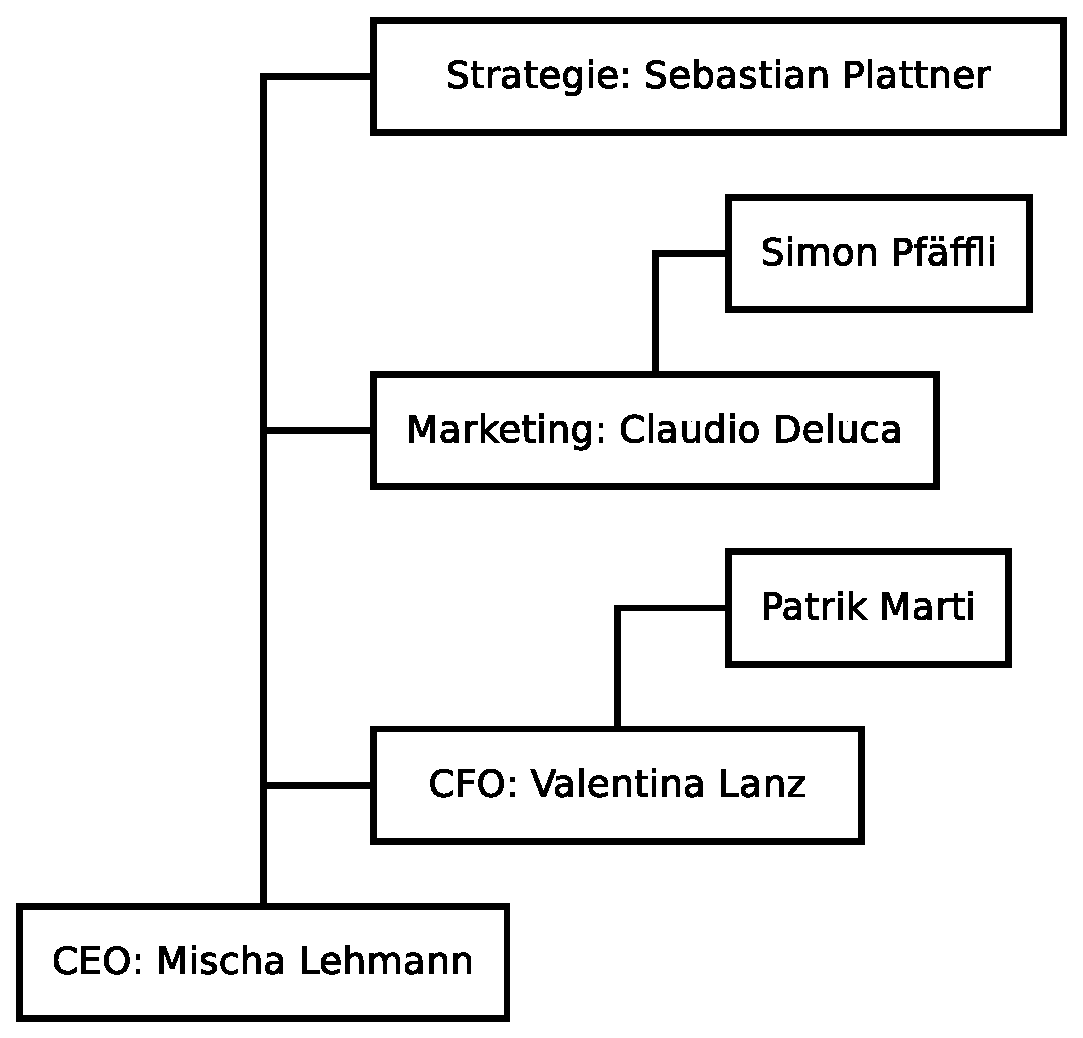
\includegraphics[scale=0.5]{bilder/organisation}
	\caption{Organigramm}
	\label{fig:organigramm}
\end{figure}

\section{Umgebungsanalyse}
\begin{center}
\begin{tabular}{ | l | l | l | } \hline
& Helpful & Harmful \\ \hline

% Internal view
\multirow{6}{*}{
\begin{sideways}
internal view
\end{sideways}}

% Internal view content
& \textbf{Strength (St�rken):} & \textbf{Weaknesses (Schw�chen):} \\ 
& ~~\llap{\textbullet}~ \underline{Einzigartigkeit}: Es werden keine �hnlichen & ~~\llap{\textbullet}~ \underline{Hohe Lohnkosten} \\
& Gadgets angeboten. & ~~\llap{\textbullet}~ \underline{Kein Eigenkapital}: Das gesamte Kapital wird \\
& ~~\llap{\textbullet}~ \underline{Starkes Management}: Wir haben ein Team & durch externe Investoren beschafft. \\
& zusammengestellt, welches in allen Gesch�fts- & ~~\llap{\textbullet}~ \underline{Erfahrung:} Wenig Erfahrung im Toiletten-Gesch�ft. \\
& bereichen gut ausgebildet ist. & \\ \hline

% External view
\multirow{8}{*}{
\begin{sideways}
external view
\end{sideways}}

% External view content
& \textbf{Opportunities (Chancen):} & \textbf{Threats (Gefahren):} \\
& ~~\llap{\textbullet}~ \underline{Marktpotenzial:} Es ist ein grosses Marktpotenzial  & ~~\llap{\textbullet}~ \underline{Produktstart:} Ein schlechter Produktstart oder \\ 
& vorhanden. Toiletten sind �berall zu finden. & Produktqualit�t k�nnte weitere Kunden vom Kauf \\
&  & unseres Produktes abhalten. \\
&  & ~~\llap{\textbullet}~ \underline{Produktnachahmer}: M�gliche Konkurrenten k�nnten  \\
&  & bei Erfolg unseres Produktes in den Markt dr�ngen. \\
&  & ~~\llap{\textbullet}~ \underline{Ruf}: Neue Kunden werden nur Interesse an userem \\ 
&  & unserem Produkt zeigen, wenn wir einen guten Ruf haben. \\ \hline
\end{tabular}
\end{center}

\section{Marktanalyse}

5 Forces

\section{Selbstanalyse}

Differential SWOT